\chapter{多特征卷积神经网络的实验结果}

\section{实验基础}

由于第三章中的实验主要是自底向上地探究网络本身的关键因素,而且通过实验可知数据增强所取得的效果最好,但是数据增强只是单纯地增加图像数量,并没有对网络属性进行改进,没有本质上的提升,该网络也不能应用在其他数据集上。所以需要从另一个角度出发,从本质上提升网络性能,提升网络的学习能力和泛化能力,使网络能够应用到其他的浮游生物数据集上,具有更强的应用性。因此,在第四章的部分有经验指导性地对网络进行改进,自顶向下地对网络进行改进提升,在浮游生物分类的相关方法和知识的基础上,将浮游生物的特征融入到卷积神经网络中,通过构造更复杂和有效的网络结构在更大的数据集上取得更好的结果。

第三章的实验结果已经证明了基于深度学习的卷积神经网络在浮游生物数据集分类上的可行性,因此这里需要在浮游生物类别更多以及图像数量更多的数据集上进行实验,保证所提出的网络模型的有效性和实际可行性,因此选择之前介绍的浮游生物图像数据集中的的WHOI-Plankton数据集。但是对于该数据集而言,虽然其所提供的浮游生物图像无论从种类和数量上都是最多的,但是缺点也是非常明显的。因此,从WHOI-Plankton数据集中,随机挑选出每类的图像数量至少有1000张的30类浮游生物图像,然后在每类中随机挑选出1000张图像,用来保证数据集的平衡性以及最终结果的可靠性。将这些浮游生物图像随机分为两部分:训练集和测试集,训练集和测试集中的图像数量比例为4:1。训练集和测试集是随机采样所得。因此,本论文所构建的Plankton数据集有30类浮游生物总共3万张图像,该数据集中的图像如图~\ref{fig:dataimages}所示,该图中的每张小图就表示一种浮游生物,其中每类的浮游生物名字显示在表~\ref{table:name}中,小图是以行优先进行排列。在这个数据集训练多特征卷积神经网络,通过实验可以证明本文所提出的基于多特征卷积神经网络在浮游生物图像分类问题上的有效性以及可拓展性。

\begin{figure}[H] % use float package if you want it here
  \centering
  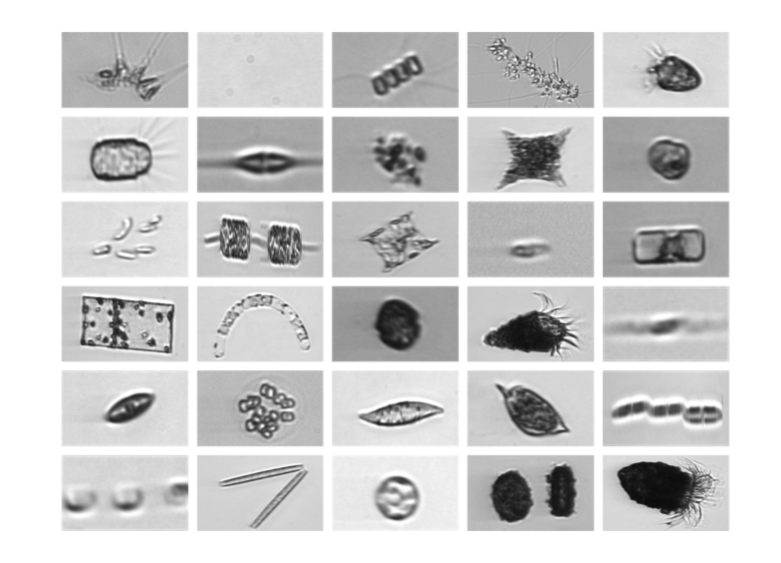
\includegraphics[height=8cm]{dataset}
  \caption{30类浮游生物的WHOI数据集中的浮游生物图像}
  \label{fig:dataimages}
\end{figure}

\begin{table}[H]\normalsize
\centering
\caption{30类浮游生物的WHOI数据集中的浮游生物类别名称}
\label{table:name}
\begin{tabular}{|c|c|c|c|}
\hline
序号 & 类别名字 & 序号 & 类别名字 \\
\hline
1 & Asterionellopsis & 16 & Guinardia\_flaccida \\ 
\hline
2 & Bad & 17 & Guinardia\_striata \\ 
\hline
3 & Chaetoceros & 18 & Heterocapsa\_triquetra \\
\hline
4 & Chaetoceros\_flagellate & 19 & Laboea\_strobila \\
\hline
5 & Ciliate\_mix & 20 & Leptocylindrus \\
\hline
6 & Corethron & 21 & Pennate \\
\hline
7 & Cylindrotheca & 22 & Phaeocystis \\
\hline
8 & Detritus & 23 & Pleurosigma \\
\hline
9 & Dictyocha & 24 & Prorocentrum \\
\hline
10 & Dino30 & 25 & Pseudonitzschia \\
\hline
11 & Dinobryon & 26 & Skeletonema \\
\hline
12 & Ditylum & 27 & Thalassionema \\
\hline
13 & Eucampia & 28 & Thalassiosira \\
\hline
14 & Flagellate\_sp3 & 29 & Thalassiosira\_dirty\\
\hline
15 & Guinardia\_delicatula & 30 & Tintinnid \\
\hline
\end{tabular}
\end{table}

本论文实验的软件环境是基于开源的深度学习框架Caffe(Convolutional Architecture for Fast Feature Embedding),硬件环境是基于四块英伟达的GTX Titan X显卡。在训练过程中,使用冲量为0.9和权值衰减系数为0.0005的随机梯度下降法。所有输出图像都会调整为256x256大小的尺寸,并且随机裁剪为227x227的大小;但是只有在原始特征图像的预处理使用减图像均值法,其他两种特征图像的预处理不需要。其他的参数初始化与AlexNet在ImageNet竞赛中使用的基本相同。

%%%%%%%%%%%%%%%%%%%%%%%%%%%%%%%%%%%%%%%%%%%%%%%%
\section{不同特征组合的分类实验结果}

为了验证多特征卷积神经网络在大数量的浮游生物图像分类上的有效性,以及该网络模型的合理性,这里同样设置多组实验对该模型进行分析与研究。多特征卷积神经网络模型同样使用 AlexNet 作为基础网络,考虑到AlexNet的训练时间、网络容量和分类准确率对于浮游生物图像分类都是比较合适的。为了考虑各种网络情况下,使用Plankton数据集上训练单网络、双网络和三网络的三组实验,在这些情况下分别对各个结果进行分析讨论:

\begin{enumerate}
\item 单特征网络AlexNet在数据集的训练

首先,只使用AlexNet分别对原始图像、全局特征图像、局部特征图像进行训练,可以得到单网络情况下AlexNet在Plankton数据集上的结果,如表~\ref{tab:single}。从表~\ref{tab:single}中可以看出,基于原始特征所训练的网络结果比基于全局特征图像和局部特征图像的网络结果都要好,可能是因为原始图像中所包含的信息更加丰富,其所训练的网络更加全面,而其他两种特征图像只包含其相对应的特征,因此所训练的网络比较片面。这里,将基于原始图像训练的AlexNet所对应的准确率94.75\%作为基础准确率,后续所有实验结果都是与该结果进行比较判断的。


\begin{table}[H]
\centering
\caption{单特征卷积神经网络在30类浮游生物图像数据上的结果}
\label{tab:single}
\begin{tabular}{|c|c|}%{|p{7cm}|p{1.8cm}<{\centering}|}
\hline
\centering{网络模型} & 准确率 \\
\hline
基于原始图像训练的AlexNet & 94.75\% \\ 
\hline
基于全局特征图像训练的AlexNet  & 94.06\% \\ 
\hline
基于局部特征图像训练的AlexNet  & 93.09\% \\
\hline
\end{tabular}
\end{table}

\item 双特征网络AlexNet在数据集的训练

因为特征融合的方法可以提升准确率,而在之前方法介绍了本方法是从多个维度对网络进行训练,因此尝试将两种不同的特征图像进行融合训练,判断网络结果最终是否得到提升。表~\ref{tab:double}表示了两种不同特征图像在Plankton数据集上的训练结果,经过原始图像信息的融合,全局特征图像和局部特征图像的训练结果都得到了提升,可能是由于原始图像信息丰富,对其余两种特征图像的信息进行了补充。而全局特征图像和全局特征图像由于之前讨论的,特征之间存在差异,较难很好地融合,因此结果几乎保持一致,没有明显提升。这里双网络的融合,是在全连接层进行矢量相连融合完成的。

\begin{table}[H]
\centering
\caption{双特征卷积神经网络在30类浮游生物图像数据上的结果}
\label{tab:double}
\begin{tabular}{|c|c|}%{|p{7cm}|p{1.8cm}<{\centering}|}
\hline
\centering{网络模型} & 准确率 \\
\hline
基于原始图像和全局特征图像训练的两个AlexNet & 95.32\% \\ 
\hline
基于原始图像和局部特征图像训练的两个AlexNet  & 94.50\% \\ 
\hline
基于全局特征图像和局部特征图像训练的两个AlexNet  & 93.33\% \\
\hline
\end{tabular}
\end{table}

\item 三特征网络AlexNet在数据集训练

对于三种特征共同训练的融合网络模型,在全连接部分可以使用直接相连的方法进行融合,但是由于不同特征之间所存在的差异,直接融合可能不会产生很好的结果。而且在全连接层中不同神经元连接数量也会有一定影响。表~\ref{tab:triple}表示三种特征训练的融合网络模型,但是没有使用交叉全连接层,而是使用最直接的全连接矢量相连的方式进行组合;另外,该表中也表示了在交叉全连接层使用不同的全连接神经元数量的影响。表~\ref{tab:triple}的结果说明了使用三种特征的网络模型相比于单特征网络模型和双特征融合网络模型,在结果上能有一定的提升。

\begin{table}[H]
\centering
\caption{全连接层设置不同,三特征融合卷积神经网络在30类浮游生物图像数据上的结果}
\label{tab:triple}
\begin{tabular}{|p{10cm}|p{1.8cm}<{\centering}|}
\hline
\centering{网络模型} & 准确率 \\
\hline
基于原始图像、全局特征图像和局部特征图像训练的三个AlexNet融合模型,没有交叉全连接层 &  95.67\% \\ 
\hline
基于原始图像、全局特征图像和局部特征图像训练的三个AlexNet融合模型,使用交叉全连接层,全连接层为4096个神经元  & 95.78\% \\ 
\hline
\end{tabular}
\end{table}


\item 基于AlexNet的多特征网络在数据集上的训练结果

本论文提出了使用原始图像、全局特征图像和局部特征图像相互融合的多特征卷积神经网络模型,在全连接层部分使用交叉全连接进行特征融合。表~\ref{tab:final}说明了使用交叉全连接的多特征融合的卷积神经网络在Plankton数据集上的实验结果。根据表~\ref{tab:triple}和表~\ref{tab:final}实验结果的比较,说明了使用交叉全连接层,可以提升准确率;另外,较少的全连接神经元,可以降低训练时间和过拟合现象,保证训练的有效性。

\begin{table}[H]
\centering
\caption{本论文所提出的多特征卷积神经网络在30类浮游生物图像数据上的结果}
\label{tab:final}
\begin{tabular}{|p{10cm}|p{1.8cm}<{\centering}|}
\hline
\centering{网络模型} & 准确率 \\
\hline
基于原始图像、全局特征图像和局部特征图像训练的三个AlexNet融合模型,使用交叉全连接层  & 95.83\% \\ 
\hline
\end{tabular}
\end{table}


\end{enumerate}

\section{网络拓展性的分类实验结果}
为了验证该多特征卷积神经网络的拓展性和实用性,这里将基础网络AlexNet替换为网络性能更好的GoogLeNet,继续进行实验。表~\ref{tab:google}表示了单特征GoogLeNet网络模型和多特征GoogLeNet网络模型在Plankton数据集上的训练结果。从表~\ref{tab:google}可知,通过网络性能更佳的GoogLeNet,相比较于AlexNet,在单网络模型上的准确率结果也有轻微提升。而对于多特征GoogLeNet网络模型在基于原始图像训练所得到的基础准确率95.2\%,也有一定程度的提升,说明了本方法的有效性。另外,由于GoogLeNet网络最后没有全连接层的存在,因此无法实现交叉全连接层。但是之前的实验已经说明了交叉全连接层的可靠性,如果这里使用交叉全连接层,最终分类准确率仍然可能还能再次提升。

\begin{table}[H]
\centering
\caption{单特征GoogLeNet网络模型和多特征GoogLeNet网络模型在30类浮游生物图像数据上的结果}
\label{tab:google}
\begin{tabular}{|c|c|}%{|p{7cm}|p{1.8cm}<{\centering}|}
\hline
\centering{网络模型} & 准确率 \\
\hline
基于原始图像训练的GoogLeNet & 95.2\% \\ 
\hline
基于全局特征图像训练的GoogLeNet  & 93.4\% \\ 
\hline
基于局部特征图像训练的GoogLeNet  & 93.2\% \\
\hline
基于三种特征图像训练的GoogLeNet  & 96.2\% \\
\hline
\end{tabular}
\end{table}

另外,为了保证实验结果的准确性,消除不确定因素等干扰,本章的实验结果已通过5次的随机交叉验证,最终的误差保证在0.1\%以内。

%%%%%%%%%%%%%%%%%%%%%%%%%%%%%%%%%%%%%%%%%%%%%%%%%%%%%%%%%%%%%%%%%%%%%
\section{本章小结}

本章节主要讨论了多特征卷积神经网络所使用的浮游生物数据集、以及多特征卷积网络模型在该浮游生物图像数据集上的分类实验结果。为了保证实验结果的合理性,本章节没有使用伍兹霍尔海洋研究所公布的WHOI-Plankton数据集,而是根据该数据集的分布特征,构建较为合理的Plankton数据集。另外,通过多组实验的设置,说明了本论文所提出的多特征卷积神经网络结构的合理性与有效性,并且将基础子网络替换,表明了该多特征网络结构具有良好的拓展性和泛化性。


